\documentclass{article}
% \usepackage{ctex}
\usepackage{mathptmx}
\usepackage[dvipsnames]{xcolor}
\usepackage{tikz}
\begin{document}
\pagestyle{empty}
% 维恩图、文氏图 Venn Diagram
% [How to draw Venn Diagrams in LaTeX](https://latexdraw.com/how-to-draw-venn-diagrams-in-latex/)
% [Example: Venn diagram](https://texample.net/tikz/examples/venn-diagram/)

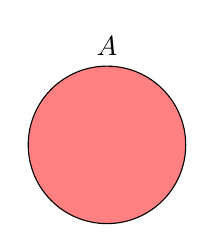
\begin{tikzpicture}
\node[draw,circle,minimum size=2cm,fill=red!50,label=$A$] (circle1) at (0,0){};     
\end{tikzpicture}

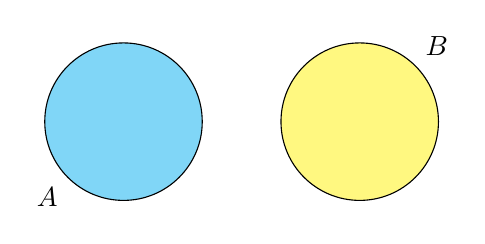
\begin{tikzpicture}
\node[draw,circle,minimum size=2cm,fill=cyan!50,label={225:$A$}] (circle1) at (0,0){};
\node[draw,circle,minimum size=2cm,fill=yellow!50,label={45:$B$}] (circle2) at (3,0){};
\end{tikzpicture}

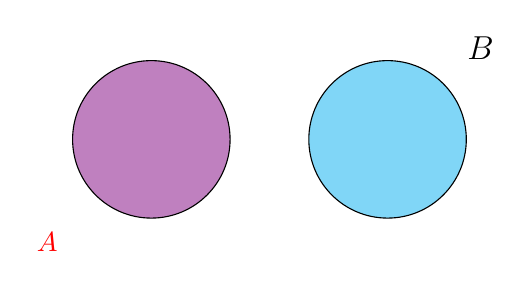
\begin{tikzpicture}
\node[draw,circle,minimum size=2cm,fill=violet!50,label={[label distance=0.5cm,red]225:$A$}] (circle1) at (0,0){};
\node[draw,circle,minimum size=2cm,fill=cyan!50,label={[label distance=0.25cm,font=\large]45:$B$}] (circle2) at (3,0){};
\end{tikzpicture}

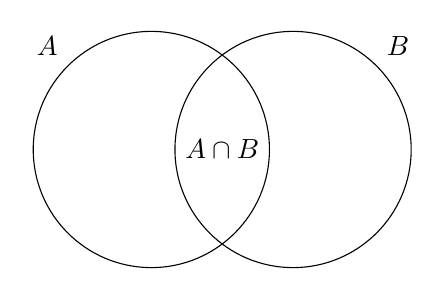
\begin{tikzpicture}
\node [draw,circle,minimum size=3cm,label={135:$A$}] (A) at (0,0){};
\node [draw,circle,minimum size=3cm,label={45:$B$}] (B) at (1.8,0){};
\node at (0.9,0) {$A\cap B$};
\end{tikzpicture}

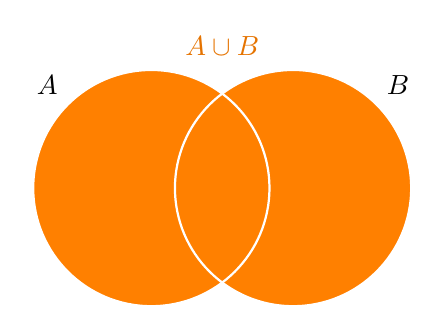
\begin{tikzpicture}
\node [circle,fill=orange,minimum size=3cm,label={135:$A$}] (A) at (0,0){};
\node [circle,fill=orange,minimum size=3cm,label={45:$B$}] (B) at (1.8,0){};
\draw[white,thick] (0,0) circle(1.5cm);
\draw[white,thick] (1.8,0) circle(1.5cm);
\node[orange!90!black] at (0.9,1.8) {$A\cup B$};
\end{tikzpicture}

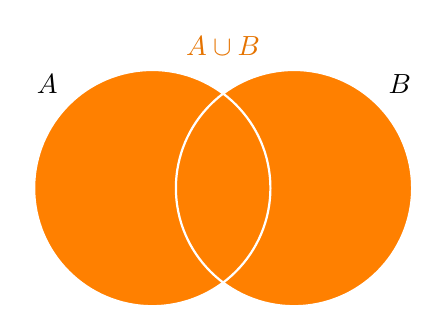
\begin{tikzpicture}[thick,set/.style={circle,fill=orange,minimum size=3cm}]
\node[set,label={135:$A$}] (A) at (0,0){};
\node[set,label={45:$B$}] (B) at (1.8,0){};
\draw[white] (0,0) circle(1.5cm);
\draw[white] (1.8,0) circle(1.5cm);
\node[orange!90!black] at (0.9,1.8) {$A\cup B$};
\end{tikzpicture}

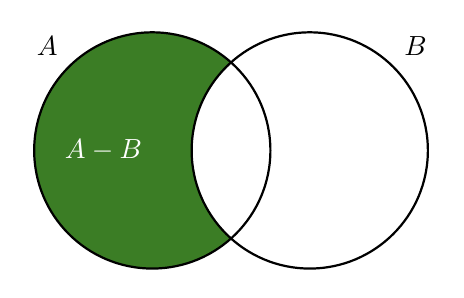
\begin{tikzpicture}[thick,set/.style={circle,minimum size=3cm}]
\node[set,fill=OliveGreen,label={135:$A$}] (A) at (0,0) {};
\node[set,fill=white,label={45:$B$}] (B) at (0:2) {};
\draw (0,0) circle(1.5cm);
\draw (2,0) circle(1.5cm);
\node[left,white] at (A.center){$A-B$};
\end{tikzpicture}

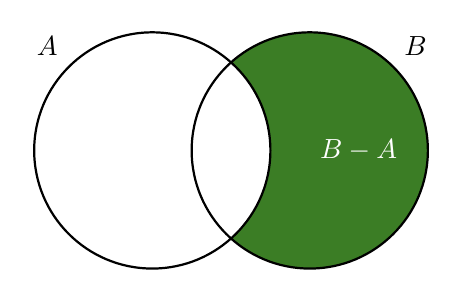
\begin{tikzpicture}[thick,set/.style={circle,minimum size=3cm}]
\node[set,fill=OliveGreen,label={45:$B$}] (B) at (0:2) {};
\node[set,fill=white,label={135:$A$}] (A) at (0,0) {};
\draw (0,0) circle(1.5cm);
\draw (2,0) circle(1.5cm);
\node[right,white] at (B.center){$B-A$};
\end{tikzpicture}

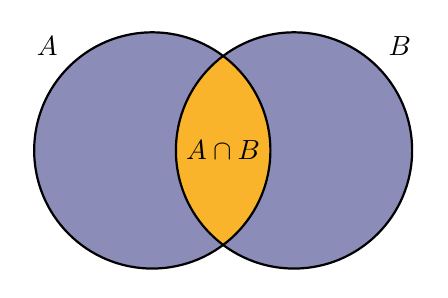
\begin{tikzpicture}[thick,set/.style={circle,minimum size=3cm,fill=MidnightBlue!50}]
\node[set,label={135:$A$}] (A) at (0,0) {};
\node[set,label={45:$B$}] (B) at (1.8,0) {};
\begin{scope}
    \clip (0,0) circle(1.5cm);
    \clip (1.8,0) circle(1.5cm);
    \fill[Dandelion](0,0) circle(1.5cm);
\end{scope}
\draw (0,0) circle(1.5cm);
\draw (1.8,0) circle(1.5cm);
\node at (0.9,0) {$A\cap B$};
\end{tikzpicture}

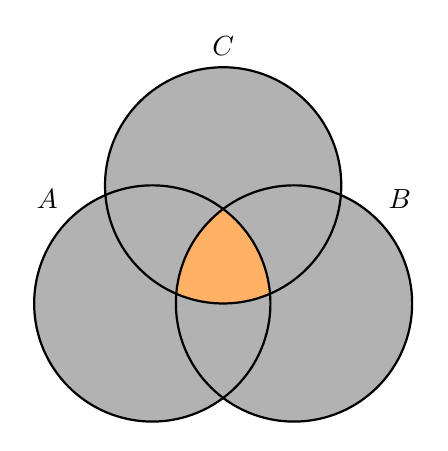
\begin{tikzpicture}[thick,set/.style={circle,minimum size=3cm,fill=black!30}]
\node[set,label={135:$A$}] (A) at (0,0) {};
\node[set,label={45:$B$}] (B) at (1.8,0) {};
\node[set,label=$C$] (C) at (0.9,1.5) {};
\begin{scope}
    \clip (0,0) circle(1.5cm);
    \clip (1.8,0) circle(1.5cm);
    \clip (0.9,1.5) circle(1.5cm);
    \fill[orange!60](0,0) circle(1.5cm);
\end{scope}
\draw (0,0) circle(1.5cm);
\draw (1.8,0) circle(1.5cm);
\draw (0.9,1.5) circle(1.5cm);
\end{tikzpicture}

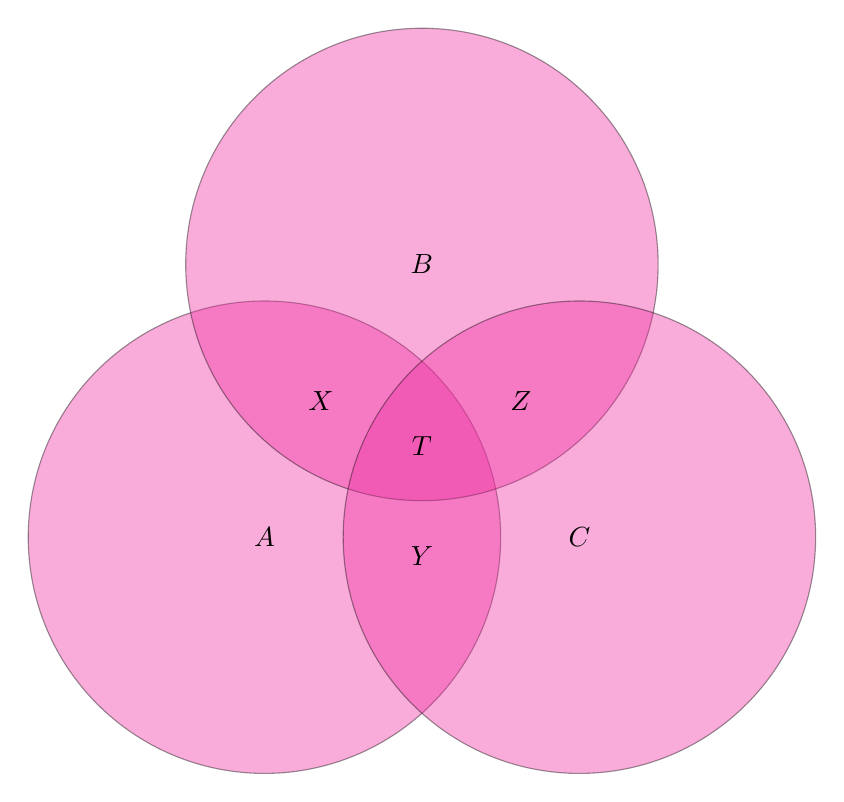
\begin{tikzpicture} [set/.style={draw,circle,minimum size=6cm,fill=Rhodamine,opacity=0.4,text opacity=1}]
\node (A) [set] {$A$};
\node (B) at (60:4cm) [set] {$B$};
\node (C) at (0:4cm) [set] {$C$};
\node at (barycentric cs:A=1,B=1) [left] {$X$};
\node at (barycentric cs:A=1,C=1) [below] {$Y$};
\node at (barycentric cs:B=1,C=1) [right] {$Z$};
\node at (barycentric cs:A=1,B=1,C=1) [] {$T$};
\end{tikzpicture}

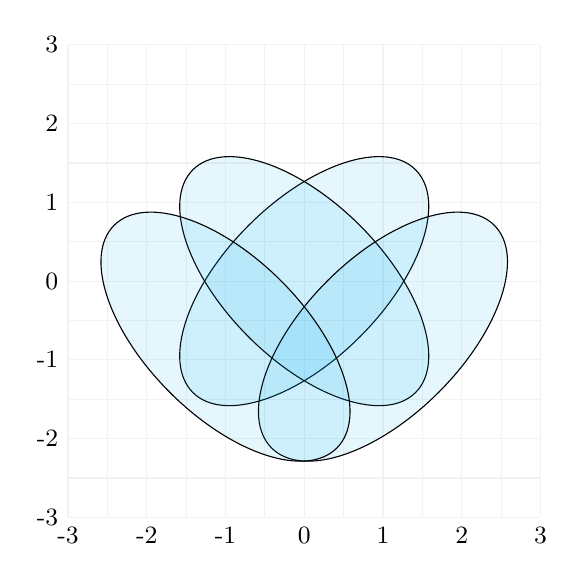
\begin{tikzpicture}[set/.style={fill=cyan,fill opacity=0.1}]
\draw[black!5,step=0.5] (-3,-3) grid (3,3);
\foreach \i in {-3,-2,...,3}
{
    \node[below] at (\i,-3){\small \i};
    \node[left] at (-3,\i){\small \i};
}
\draw[set,rotate=45] (0,0) ellipse (2cm and 1cm);
\draw[set,rotate=-45] (0,0) ellipse (2cm and 1cm);
\draw[set,xshift=1cm,yshift=-0.705cm,rotate=45] (0,0) ellipse (2cm and 1cm);
\draw[set,xshift=-1cm,yshift=-0.705cm,rotate=-45,] (0,0) ellipse (2cm and 1cm);
\end{tikzpicture}


\def\firstcircle{(0,0) circle (1.5cm)}
\def\secondcircle{(45:2cm) circle (1.5cm)}
\def\thirdcircle{(0:2cm) circle (1.5cm)}

\begin{tikzpicture}
\draw \firstcircle node[below] {$A$};
\draw \secondcircle node [above] {$B$};
\draw \thirdcircle node [below] {$C$};

\begin{scope}
    \clip \firstcircle;
    \fill[red] \secondcircle;
\end{scope}

\begin{scope}
    \clip \firstcircle;
    \clip \secondcircle;
    \fill[green] \thirdcircle;
\end{scope}

\begin{scope}[shift={(6cm,0cm)}]
    \begin{scope}[even odd rule]
        \clip \secondcircle (-3,-3) rectangle (3,3);
        \fill[yellow] \firstcircle;
    \end{scope}
    \draw \firstcircle node {$A$};
    \draw \secondcircle node {$B$};
\end{scope}

\begin{scope}[shift={(3cm,-5cm)}, fill opacity=0.5]
    \fill[red] \firstcircle;
    \fill[green] \secondcircle;
    \fill[blue] \thirdcircle;
    \draw \firstcircle node[below] {$A$};
    \draw \secondcircle node [above] {$B$};
    \draw \thirdcircle node [below] {$C$};
\end{scope}
\end{tikzpicture}

\end{document}